\section{Partie théorique}

\subsection{Reseau Sémantique}

L'ambiguité inhérent des langues humaines est un grand défi pour le traitement automatique
de langue naturelle. En linguistique, même s'il y a beaucoup d'avances dans la
désambiguisation syntaxique, l'ambiguité sémantique reste une tâche extrèment difficile.
Un supercomputer Watson de IBM a réussi a gagné a Jeopardy avec toute sa
puissance mais sans eviter de faire des fautes simples. En plus, la répresentation
sémantique logique n'est toujours pas au point de résoudre des tâches qui ont
besoin des liens moins concrète ou plus flous, telles que
\begin{itemize}
\item la désambiguïsation lexicale (Word Sense Disambiguation)
\item la recherche d'information (par exemple sur la toile ou dans une bibliothèque)
\item la catégorisation de documents
\item le résumé automatique de texte
\item la traduction automatique
\end{itemize}
L'idée le plus populaire pour résoudre ses difficultés est l'utilisation d'un réseau
sémantique qui donne l'avantage de pouvoir répresenter tous les connections taxonomiques
ensembles en une seule entité. Cette simplication n'est pas sans coût, en particulier
la répresentation des liens logiques telles que la négation et la disjonction 
et en plus connaissances non-taxonomique sont particulièrement difficile à capter.

L'idée de base pour un reseau semantique est de construire un graphe avec
les concepts pour noeuds et les liens entre les concepts comme arrêts.
Il exist deux approches générales à la construction. Premièrement, à
partir d'un dictionnaire, et deuxièment, à partir d'un corpus.
Un corpus a l'avantage de contenir les vraies utilisations des mots non-biasé
par les selections des auteurs, et aussi une grande
quantité d'utilisations, mais au même temps exige un algorithme non-supervisé pour la
désambiguisation et un autre algorithme pour la conversion de collocation en lien sémantique.
Word2Vec \hyperref[bib:word2vec]{[~\ref*{bib:word2vec}]} de
google réprésente le point actuel de cet approche.
Par contre, le dictionnaire, même si plus petit, donne plus
d'information sur les mots rares et possède déjà des liens sémantiques explicites entre
les mots.

\subsection{Structure du reseau}

L'utilisation d'un dictionnaire dans les tâches semantiques computationnelles
existe depuis les années 60 \hyperref[bib:olnyetal]{[~\ref*{bib:olnyetal}]}.
La construction d'un réseau sémantique à partir d'un dictionnaire (par exemple
en français \hyperref[bib:gaumeetal]{[~\ref*{bib:gaumeetal}]},
\hyperref[bib:mulleretal]{[~\ref*{bib:mulleretal}]}) est possible 
grâce à la structure des dictionnaires qui permet de faire ressortir des liens 
sémantiques. La structure en sens, sous-sens, définitions, et exemples, parmi 
d'autres informations, mais aussi la structure interne des définitions contient 
une régularité qu'il est important d'exploiter au maximum. Nous tenons donc à 
conserver le plus possible cette structure dans la transformation de dictionnaire 
en graphe. Un graphe est défini formellement comme un ensemble de sommets et un 
ensemble d'arcs qui relient une paire de sommets.

\[
G = <S, A>
\]

Pour représenter un dictionnaire par un graphe, nous considérons que les 
sommets peuvent être les mots individuels du dictionnaire ou même les niveaux 
intermédiaires de la structure tels que `exemple', `définition', `synonyme', 
`antonyme' etc. Les arcs sont alors les liens qui lient les différents éléments 
d'une entrée de dictionnaire et permettraient de trouver un lien entre un 
lexème donné et la manière dont il est décrit dans son entrée du dictionnaire.

Le graphe d'un reseau sémantique est connu d'exhiber les propriétés `Small World'
\hyperref[bib:veronis]{[~\ref*{bib:veronis}]} -
terme qui existe depuis l'experience fameux de Travers et Milgram
\hyperref[bib:traversmilgram]{[~\ref*{bib:traversmilgram}]}.
Watts et Strogatz \hyperref[bib:wattsstrogatz]{[~\ref*{bib:wattsstrogatz}]}
ont défini les propriétés d'un graphe `Small World' ainsi:
Si un graphe possède $N$ noeuds, et $d_{min}(i,j)$ est la distance minimum
entre noeuds $i$ et $j$, le `Characteristic Path Length' $L$ se défini par:
$$L = \frac{1}{N(N-1)} \sum\limits_{i\ne j} d_{min}(i,j) $$
et si pour un noeud $i$, l'ensemble de ses voisins immédiats est $\Gamma (i)$
et le nombre d'arrêts entre ses voisins immédiats est $E(\Gamma (i))$
alors le `Clustering Co-efficient' $C$ se défini par:
$$C = \frac{1}{N}\sum\limits_{i=1}^N \frac{E(\Gamma (i))}{\binom{|\Gamma (i)|}{2}} $$
Autrement dit, $L$ est la moyenne des distances minimales entre chaque couple
de noeuds dans le graphe, et $C$ est la moyenne du ratio des liens entre les voisins d'un
noeud et le nombre maximum de liens possible.

Un graphe `Small World' est défini par les propriétés suivants:
$$L \sim L_{rand} \sim \frac{log(N)}{log(k)} $$
et
$$C >> C_{rand} \sim \frac{2k}{N} $$
où $k$ est le dégée moyenne des noeuds du graphe et $L_{rand}$ et $C_{rand}$ sont respectivement
le Characteristic Path Length et Clustering Co-efficient pour un graphe aléatoire.

Par conséquent, un graphe `Small World' n'est pas dense, mais a des distances entre les noeuds
très petites. Une autre conséquence démontré par Barabási et Albert
\hyperref[bib:barabasi]{[~\ref*{bib:barabasi}]} est que la distribution des dégrés
des noeuds suivre une loi de puissance:
$$ p(k) \propto k^{-\alpha}$$
où $p(k)$ est la probabilité d'un noeud quelconque d'avoir un dégré k, et
$\alpha$ s'approche à l'unité (\hyperref[bib:veronis]{[~\ref*{bib:veronis}]}). Dans les
figures \hyperref[fig:ndefinitionsperentry] et \hyperref[fig:nmotsperentry], cette
comportement est visible pour le Littré dictionnaire.

% make histograms here
\begin{figure}
\begin{center}
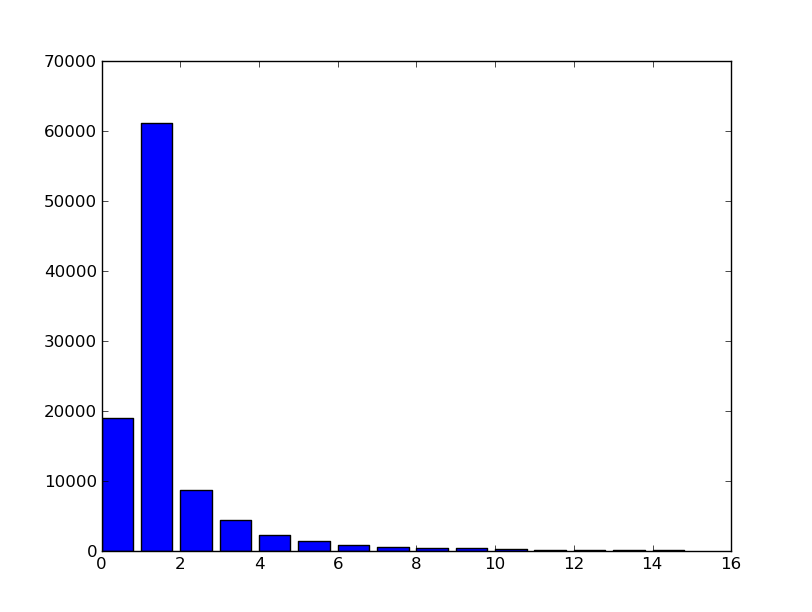
\includegraphics{Images/definitions_per_entry_cat.png}
\caption{Le nombre de définitions par entrée plus catégorie dans le Littré,
parfois une catégorie manque une
défintion et a seulement une référence d'où les zéros.}
\label{fig:ndefinitionsperentry}
\end{center}
\end{figure}

\begin{figure}
\begin{center}
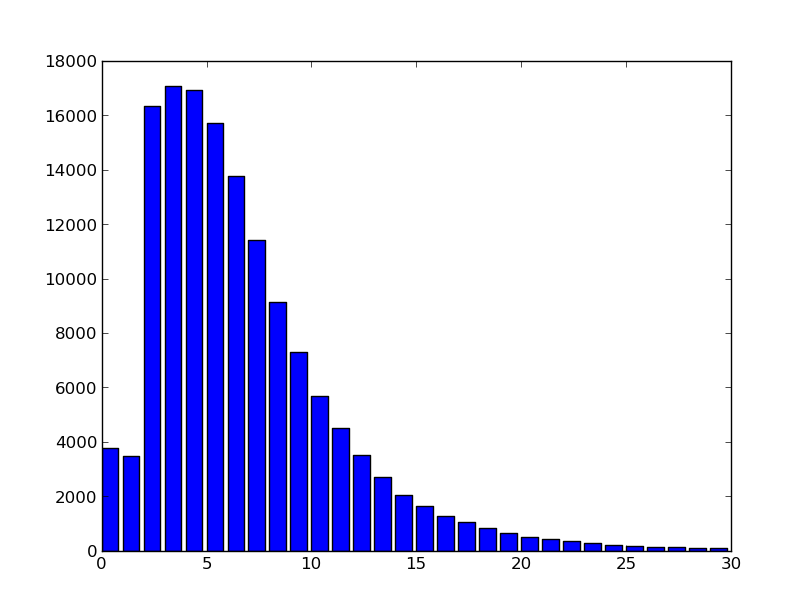
\includegraphics{Images/words_in_definitions.png}

\caption{Le nombre de mots lexicaux par définition le Littré}
\label{fig:nmotsperentry}
\end{center}
\end{figure}

Un problème qui se présente dans un reseau sémantique est comment d'évaluer une distance
entre un noeud et un ensemble de noeuds, ou même entre deux ensembles de noeuds. La
première situation peux se passer dans la classification des textes, où on veut lier
l'ensemble de mots dans un texte à une classification sémantique pertinente. La
deuxième situation se voit dans la désamigüisation lexicale, où il y une définition
composé d'un ensemble de mots qu'on veut comparer avec un contexte, aussi composé
d'un ensemble de mots.

L'algorithme Lesk \hyperref[bib:lesk]{[~\ref*{bib:lesk}]} est une solution possible pour
resoudre ce problème. Il se fait par le chevauchement de deux ensembles de mots, dans
le cas d'un seul mot, sa définition dans le dictionnaire est utilisé. Clairement ce
methode est très sensible aux mots dans la définition utilisé, et aussi ne donne
pas un résultat s'il n'y a pas de chevauchement entre les deux ensembles. 

\subsection{ Marche Aléatoire }

Avec la construction d'un reseau sémantique, la notion de distance peut se définir
dans plusieurs manières. Evidamment, entre 2 noeuds $i$ et $j$, on peut prendre 
la métrique de la distance la plus courte parmi les chemins qui mènent de $i$ a 
$j$. Un problème avec cette approche se voit facilement avec un simple carré ( 
\hyperref[fig:square] )

\begin{figure}[!ht]
\centering
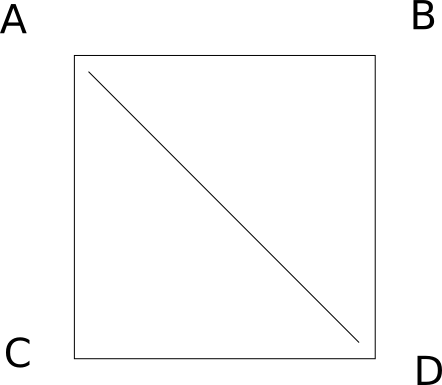
\includegraphics{Images/square.png}
%\def\svgwidth{\columnwidth}
%\input{Images/square.pdf_tex}
\caption{Un simple reseau avec 4 noeuds}
\label{fig:square}
\end{figure}

Si le lien A-D existe, alors il va probablement définir la distance A-D, mais s'il n'existe pas,
soit le chemin A-B-D, soit le chemin A-C-D va le déterminer. Donc si un lien 
direct est explicite ou non peut influencer la distance entre les noeuds. 
Ainsi, si une définition n'inclue pas un mot qui est sémantiquement proche, la 
distance risque d'être mal representée. En plus la distance la plus courte ne 
prend pas compte de la diversité des chemins qui peuvent lier deux noeuds.

Pour ces raisons, il est possible de proposer une alternative metric de distance en interpretant
le reseau comme une chaîne de Markov \hyperref[bib:mulleretal]{[~\ref*{bib:mulleretal}]}.
L'entrée $(i,j)$ dans la  matrice d'adjacence est donc
proportionelle à la probabilité d'une transition de noeud $i$ en noeud $j$. Pour pouvoir interpretter
ces transitions comme des probabilités il faut les normaliser:

$$p(i\rightarrow j) = \frac{M_{i,j}}{\sum\limits_{k} M_{i,k}}$$

En multipliant un vecteur d'un état $i$ par la matrice à la puissance $t$, on obtien un vecteur
qui réprésente la probabilité d'être à chaque noeud après un nombre de pas $t$. Pour une graphe
fortement connexe, si $t$ est grand,
cette distribution s'approche à un equilibrium ou point stable où le flou de probabilité vers
un noeud est égal au flou sortant. Cette idée est le coeur de l'algorithme pagerank
\hyperref[bib:pagerank]{[~\ref*{bib:pagerank}]},
utilisé par Google pour donner un rang à chaque page dans le graphe de l'internet.

Une difficulté pour pagerank est de gérer la structure du web lui-même, illustré en
figure \hyperref[fig:webstructure]. Le coeur est un component fortement connexe (scc), il y a
aussi une grande partie ``In Component'' qui a seulement les liens dirigés vers le scc
et une deuxième grande partie ``Out Component'' qui ne possède des liens sortants mais
est la destination des autres liens. Les tendrils, tubes et autres components déconnectés
entièrements font une portion plus petite. L'algorithme de pagerank va voir après du temps
toute la probabilité piégé dans les endroits sans sortie, d'où le besoin du `taxation',
c'est-à-dire la redistribution d'une proportion de probabilité $Beta$ après chaque
multiplication de $M$. Donc nous avons:
$$ p(t+1) = \beta*M*p(t) + (1-\beta)*v$$
où $v$ est un vecteur composé completement de valeurs $1$, au lieu de
$$ p(t+1) = M*p(t)$$ 

\begin{figure}[!ht]
\centering
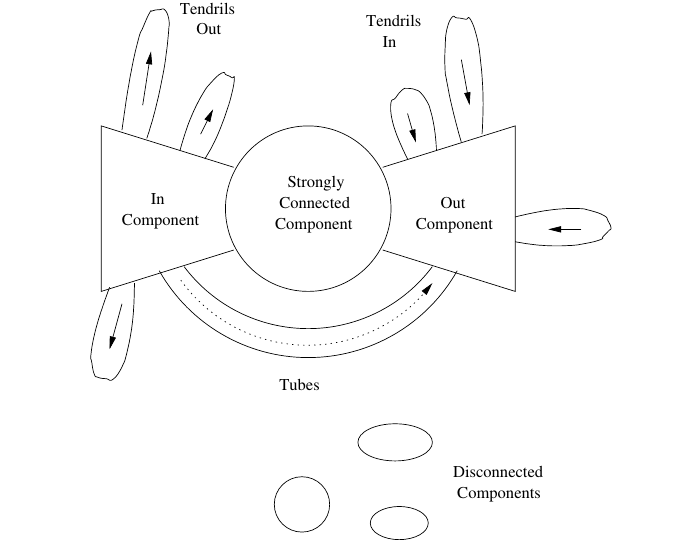
\includegraphics{Images/web_graph_structure.png}
\caption{Le structure de la toile, image pris de
\hyperref[bib:linkanalysis]{[~\ref*{bib:linkanalysis}]}}.
\label{fig:square}
\end{figure}

Après un nombre d'itérations $t$ qui est large, il y aura de nouveau un point stable,
mais sans la probabilité entièrement dans les pièges. Le paramètre $Beta$ est normalement
choisi d'être  $\approx 0,85$. De plus, il est possible de calculer une probabilité
biasé par le point d'origine si, au lieu de $v$, on met $v'$ qui a un ensemble de
noeuds a $1$, et le reste à $0$.

La structure du graphe orienté du dictionnaire ressemble beaucoup à celui de la toile,
et alors on peut utiliser les mêmes méthodes et algorithme pour calculer la distance
d'un ensemble de mots vers un seul autre ou un groupe d'autre noeuds.


\subsection{Remarques sur la terminologie}
Nous appelons `mot' toute unité minimale du lexique. Un mot peut être
soitfléchi, soit non-fléchi et par défaut nous faisons référence aux mots 
non-fléchis sous leur forme de dictionnaire. Par principe, nous restreignons le 
réseau aux lemmes, mais il est possible qu'il y apparaît des formes fléchies en 
cas de non-identification du lemme.

Par `entrée' de dictionnaire nous faisons référence à un groupe d'informations 
(catégories syntaxiques, sens, définitions, exemples etc.) associées à un mot 
donné. Par conséquent, le terme `entrée' peut aussi être utilisé pour dénoter 
le mot lui-même, et par extension les informations contenues pour ce mot donné.

La relation sémantique de synonymie est définie entre deux termes de la même 
catégorie de discours qui ont le même sens et qui peuvent donc être substitués 
l'un pour l'autre sans modifier le sens de la phrase. Cette définition pose 
évidemment des problèmes, surtout à cause du fait qu'il est toujours possible 
de trouver une différence de sens ou d'usage entre deux mots malgré le fait 
qu'ils soient habituellement classés en synonymes. Il est parfois souhaitable 
de parler de proche-synonymes au lieu de synonymes tout court. Néanmois, 
nous préférons utiliser le terme `synonyme' pour parler de ces cas, sans 
postuler de théorie sur les frontières de la synonymie. Par la suite, la 
synonymie sera définie en termes de relations attestées dans des ressources 
externes et nous nous reportons à ces références pour établir si deux mots sont 
en relation de synonymie ou pas.

De même pour les relations d'antonymie, d'hyperonymie et d'hyponymie. 
L'antonymie est définie comme la relation entre deux mots à sens opposé. 
L'hyperonymie entre un mot dont l'extension contient l'extension d'un autre mot 
(par exemple, `véhicule' est l'hypernym de `voiture'). L'hyponymie est la 
relation inverse d'hyperonymie, entre un mot dont l'extension est incluse dans 
l'extension d'un autre (pour reprendre le même exemple, `voiture' est un 
hyponyme de `véhicule').

[AUTRES DEFINITIIONS...]
